% Appendix A

\chapter{Apéndice Planos de rotadores} % Main appendix title

\label{AppendixA} % For referencing this appendix elsewhere, use \ref{AppendixA}

\lhead{Appendix A. \emph{Planos de las piezas de rotadores.}} % This is for the header on each page - perhaps a shortened title

\graphicspath{{Figures/planos_piezas_rotador/}{../Figures/planos_piezas_rotador/}} 

El ensamble de la Fig. A.1 muestra los tres elementos diseñados y
fabricados en el contexto del proyecto de grado, y en seguida se adjuntan los planos de
fabricación de cada uno. Estos son, (a) la placa metálica sobre la cual se
soportan los otros elementos, (b) la montura sobre la cual está
empotrado un rodamiento de bolas, y (c) un buje de bronce que entra a
presión en el rodamiento y sobre el cual se atornillan las monturas de
placas retardadoras y polarizadores. 

\begin{figure}
\centering
\label{fig:plano_ensamble}
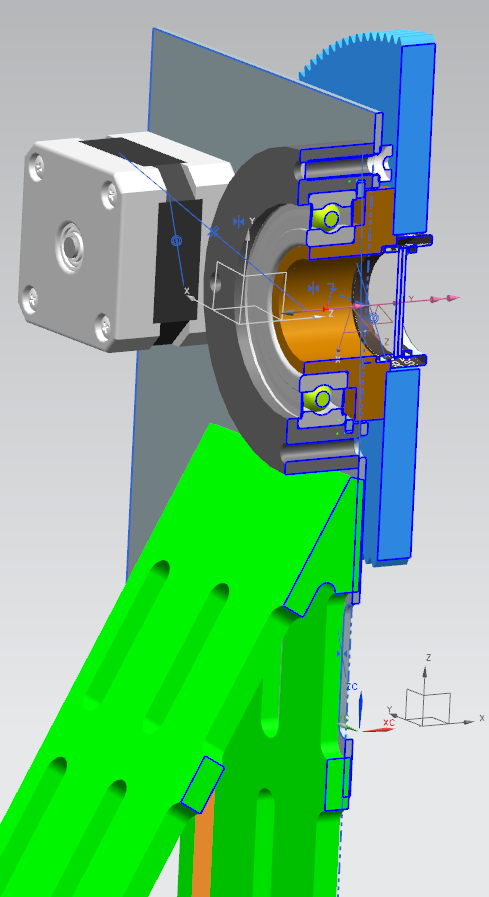
\includegraphics[scale = .8]{Montaje.png} 
\caption[Corte transversal del ensamble de los rotadores de elementos
ópticos]{Corte transversal del ensamble de los rotadores de elementos
  ópticos. (a) Placa soporte en lámina de aluminio calibre 11, (b)
  montura para rodamiento en bronce, y (c) buje roscado para monturas
  de polarizadores y retardadores. }
\end{figure}
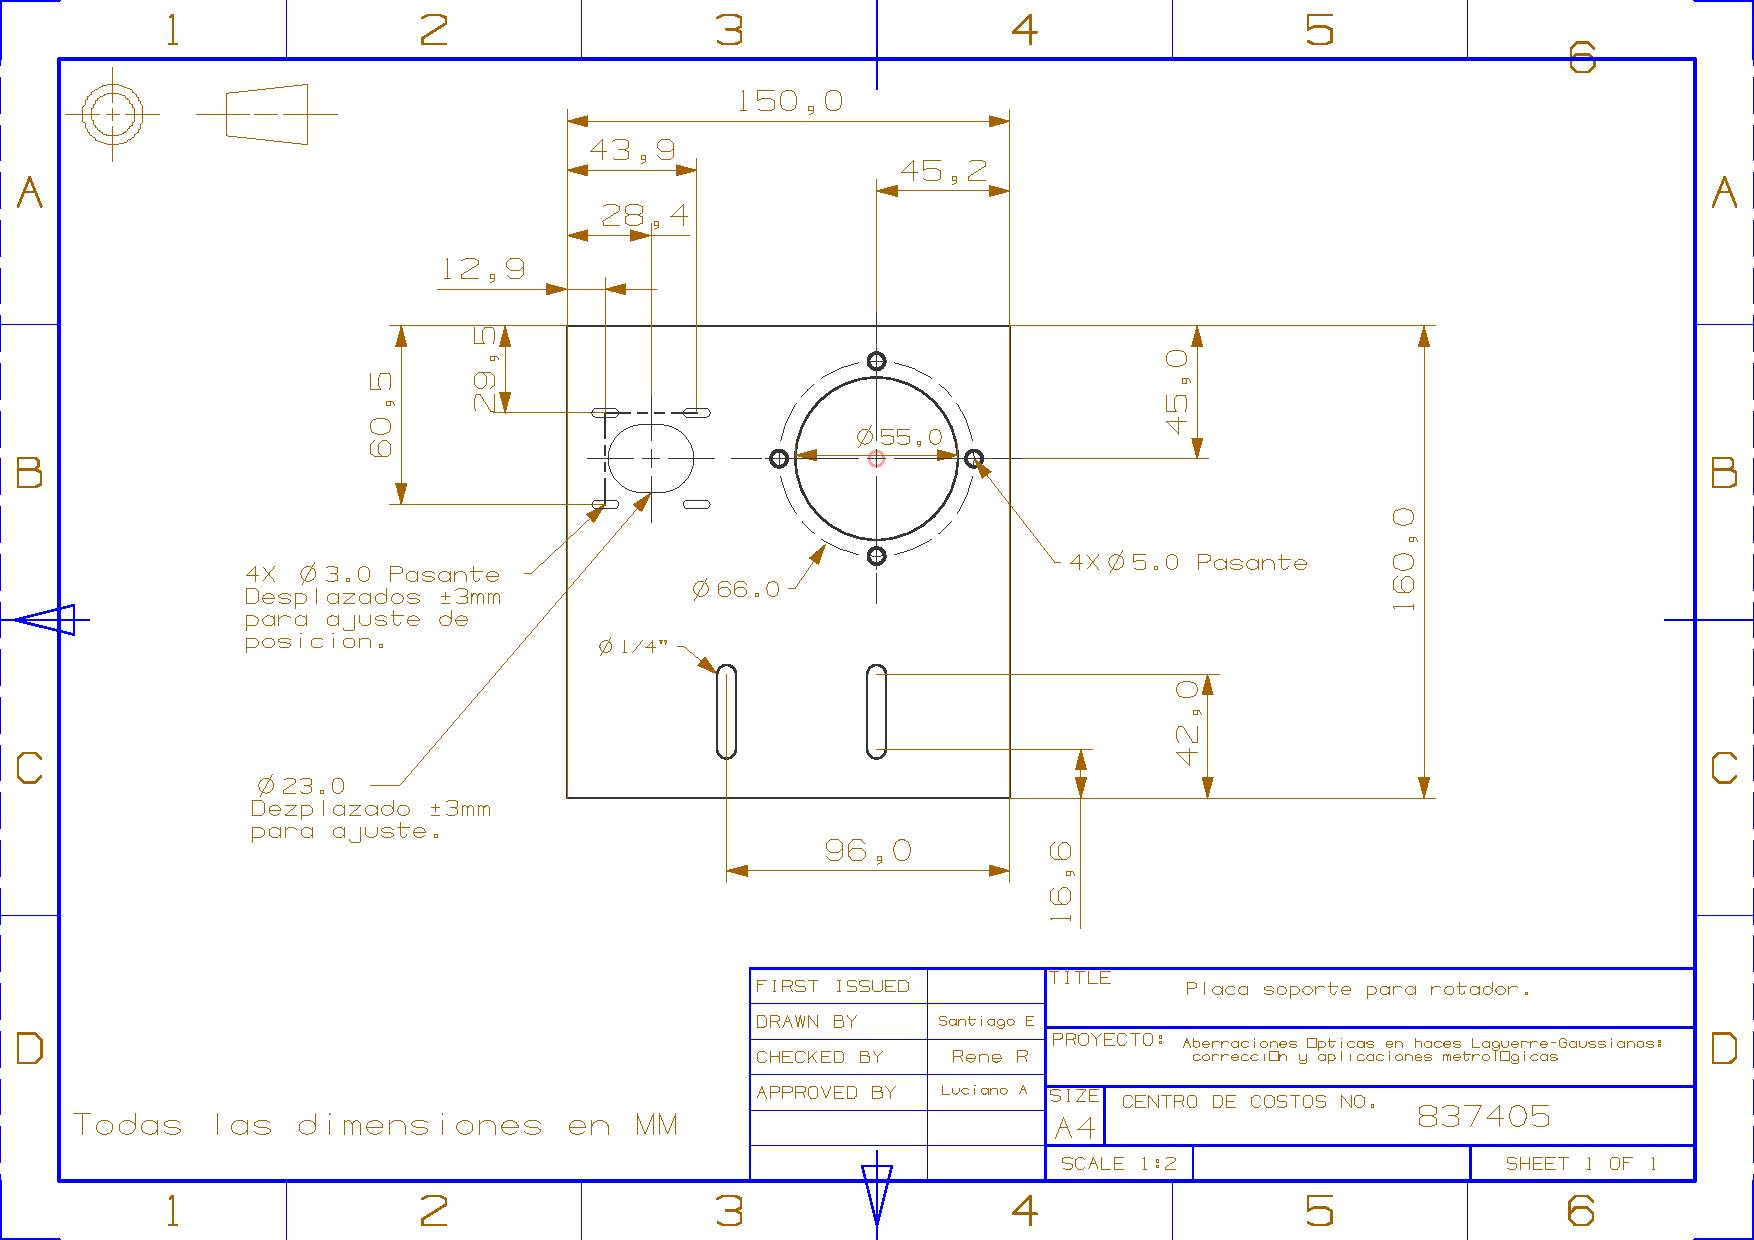
\includepdf[pages={1},landscape=true]{placa_soporte.pdf}
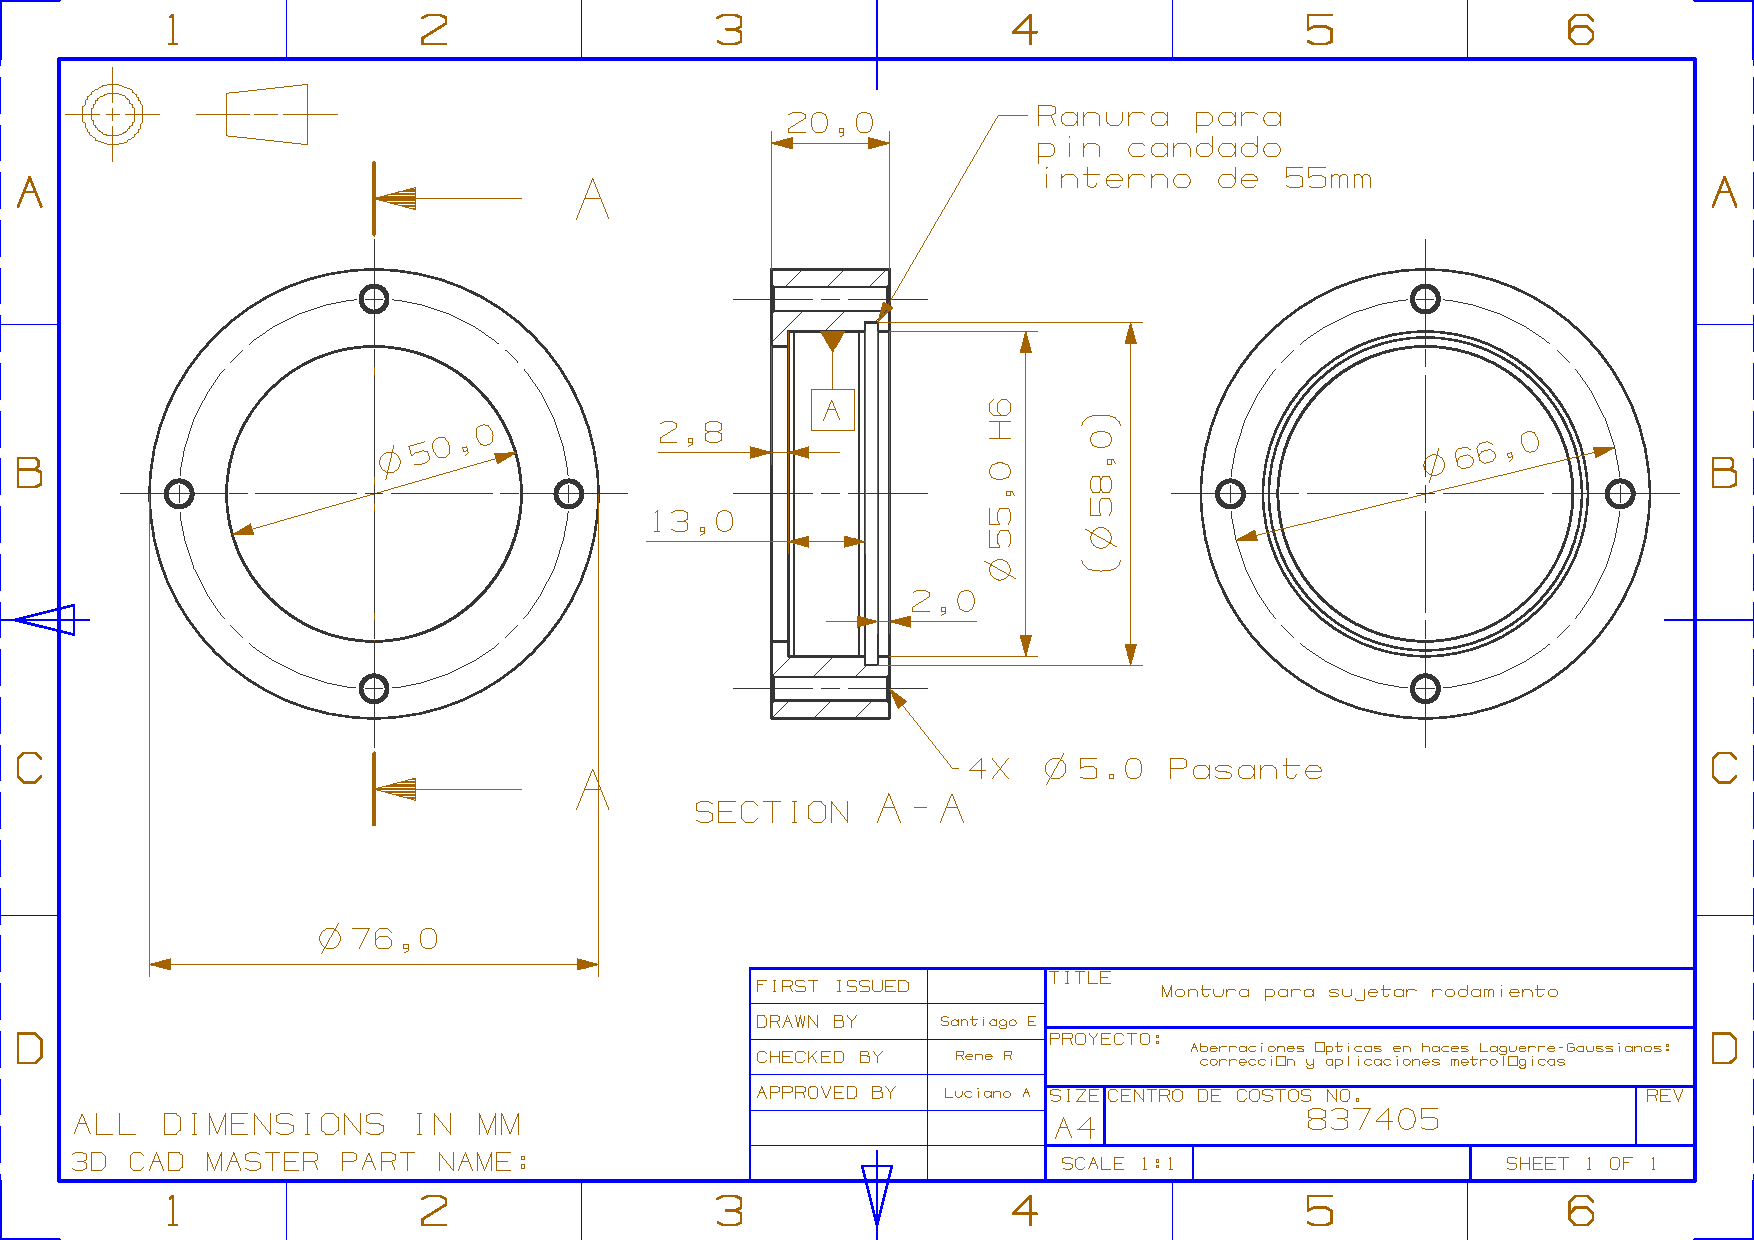
\includepdf[pages={1},landscape=true]{montura.pdf}
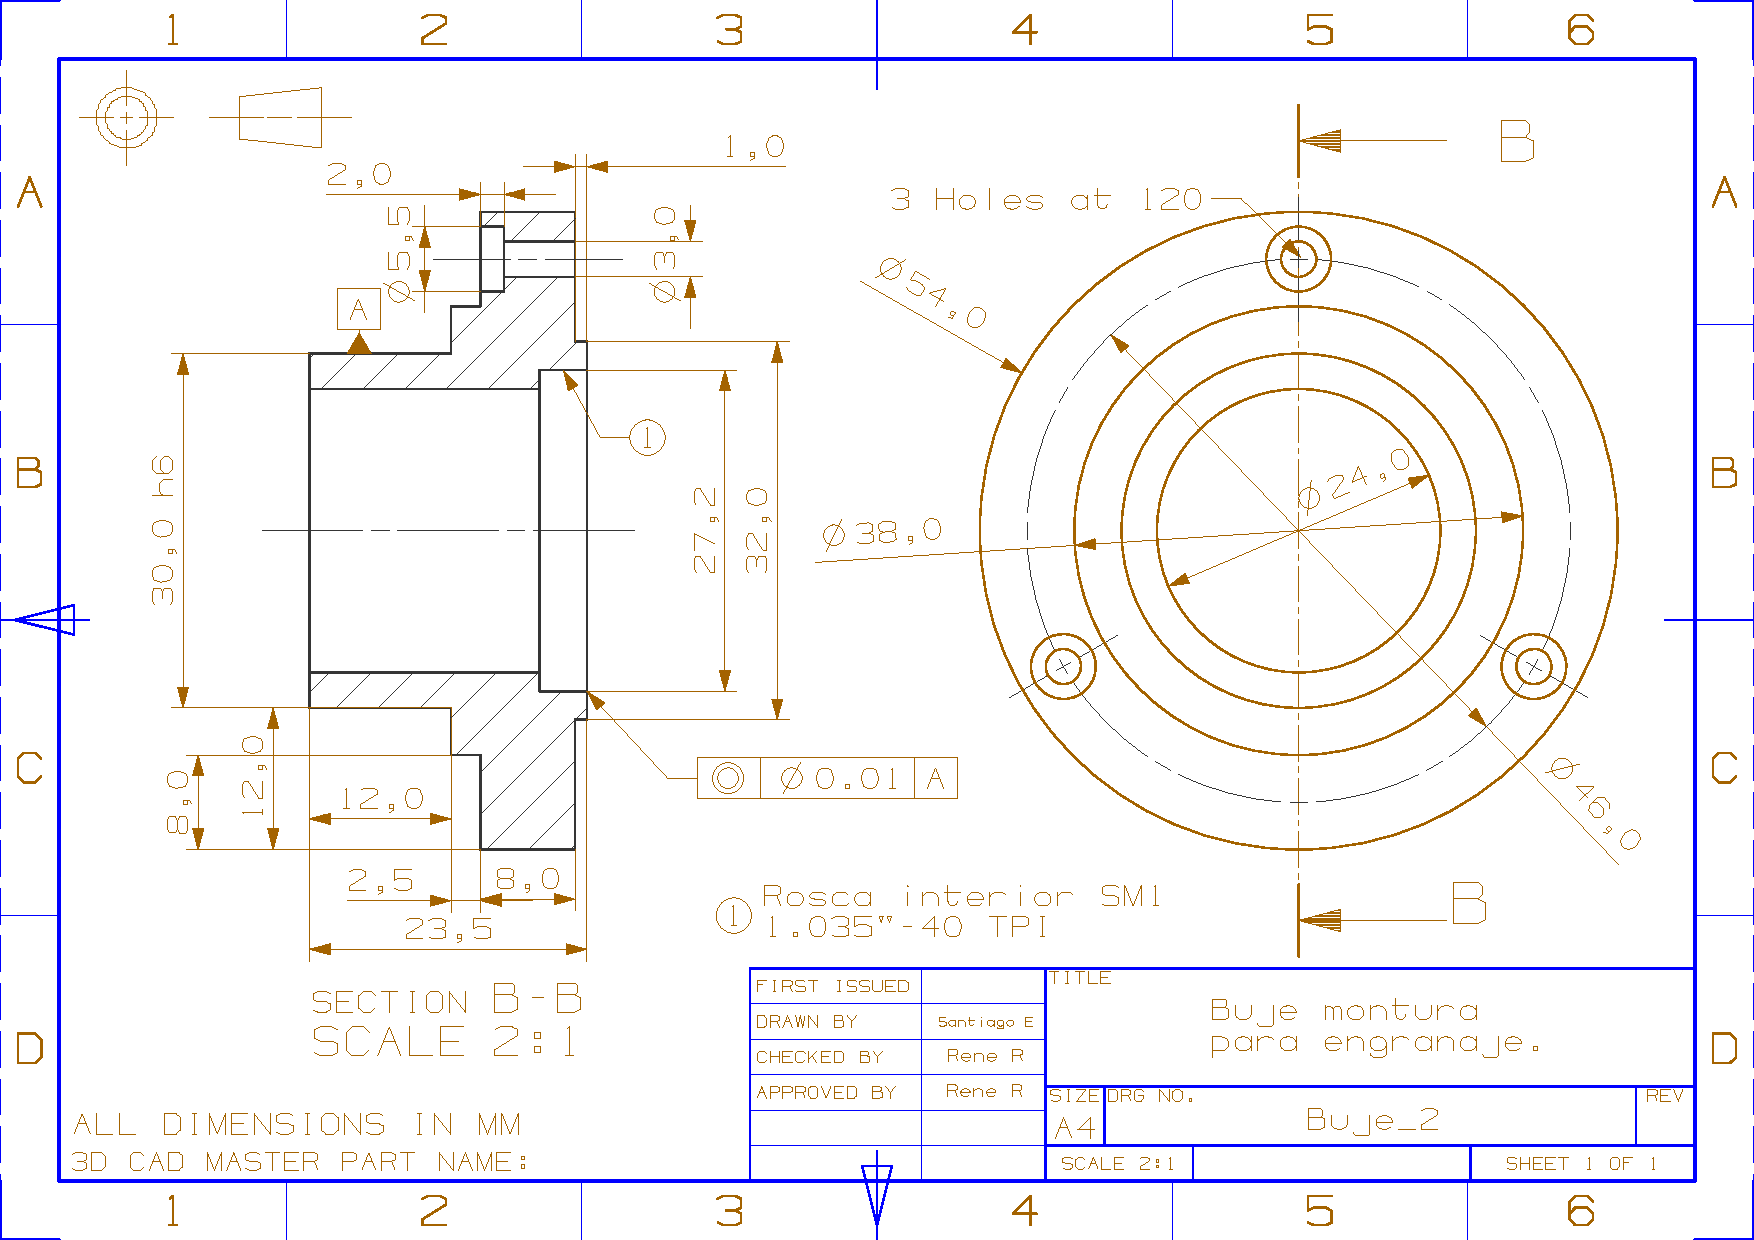
\includepdf[pages={1},landscape=true]{design.pdf}

